\documentclass{dingjia}

\ctexset{autoindent=false}
\setlength\parindent{0pt}

\hypersetup{%
  colorlinks = true,
  citecolor=magenta,
  linkcolor=blue,
  bookmarksnumbered = true,
  bookmarksopen = true,
  pdfcreator = {sd44sd44@yeah.net},
  pdfauthor = {蛋疼的蛋蛋},
  pdfsubject = {数据库系统概念 形式化关系查询语言习题},
}
\usepackage{minted}
\usemintedstyle{perldoc}

\begin{document}

\begin{figure}[ht]
  \centering
  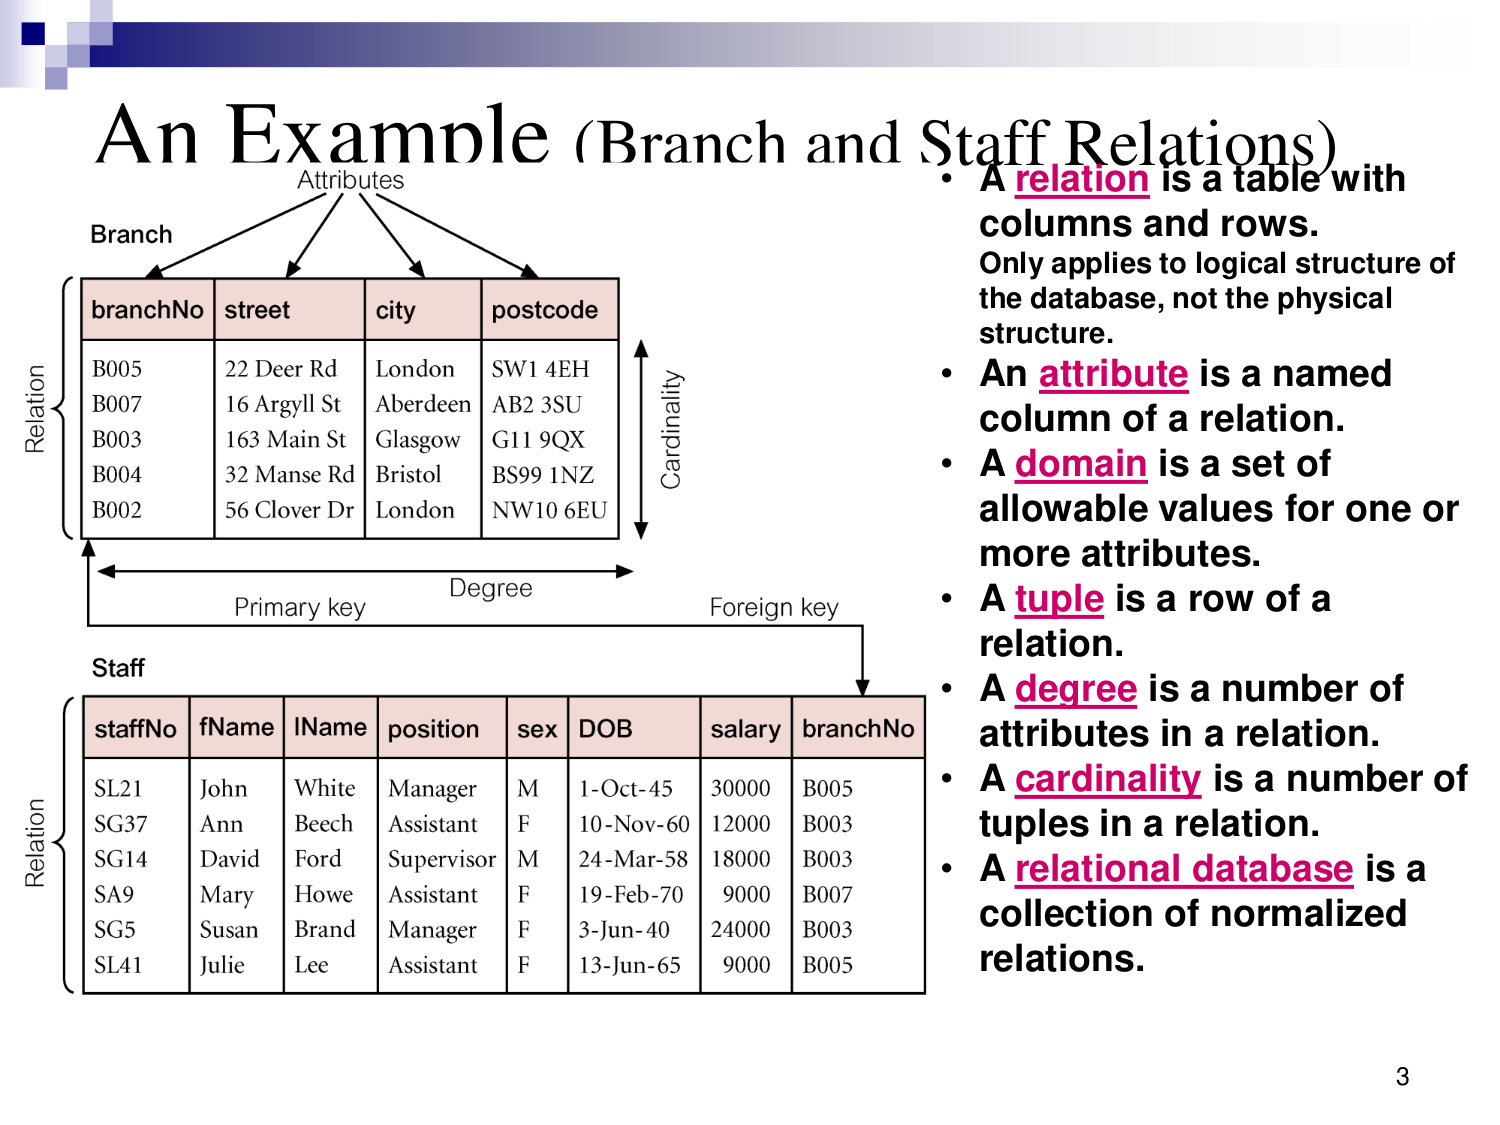
\includegraphics[width=0.8\textwidth]{img/sqlNorn.png}
  \caption{\label{fig:sqlnorn}SQL名词解释(瓦莱腊大学讲义) }
\end{figure}

\begin{figure}[ht]
  \centering
  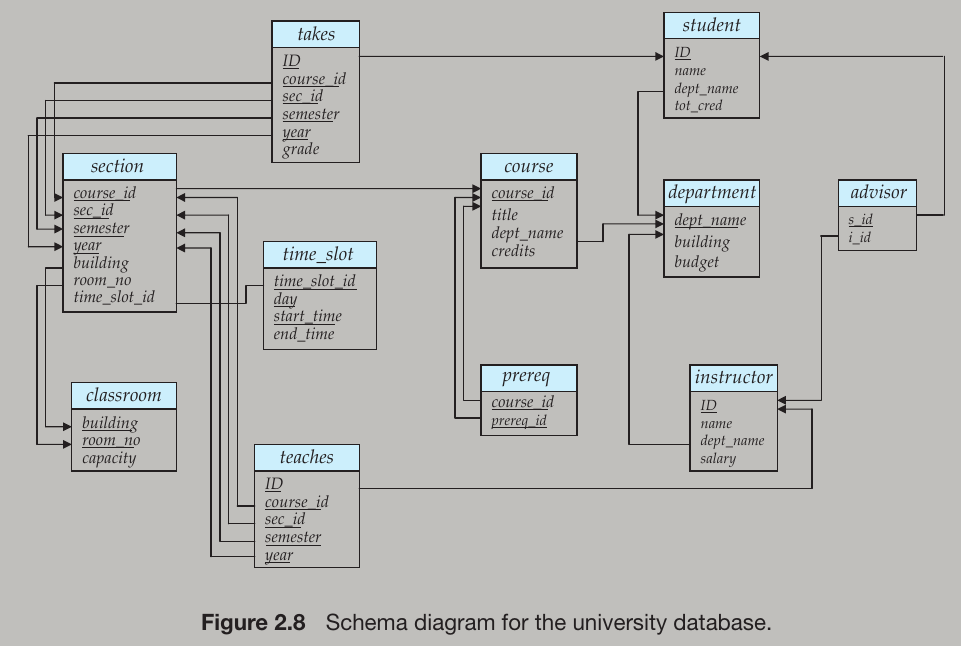
\includegraphics[width=0.8\textwidth]{img/schoolmodel.png}
  \caption{\label{fig:school}本书学校数据库模式图 }
\end{figure}

一些有用的链接:
\begin{itemize}
\item \href{https://en.wikipedia.org/wiki/Relational\_algebra}{维百:关系代
    数}
\item \href{https://en.wikipedia.org/wiki/Domain\_relational\_calculus}{维百:域关系演算}
\item \href{http://mit.wu.ac.th/mit/images/editor/files/db-lecture03-2013.pdf}{瓦来腊大学讲义}
\item \href{https://cs.nyu.edu/~jcf/classes/CSCI-GA.2433-001_sp15/slides/session5/RelationalAlgebra-RelationalCalculus-SQL.pdf}{纽约大学讲义}
\end{itemize}


\begin{enumerate}
\item 使用大学模式,用关系代数来表达下面这些查询
  \begin{enumerate}
  \item 找出计算机系开设的占3个学分的课程的名称
    \[ \Pi_{title}(\sigma_{dept\_name = "Comp.\ Sci." \land credits = 3}(instructor))\]

  \item 找出选了教师Einstein所教课程的所有学生的ID,注意结果中不能有重复。
    \[\Pi_{id}(takes \bowtie \Pi_{course\_id}(\sigma_{name = "Einstein"}(instructor \bowtie teaches)))\]

    此题官网答案有个无伤大雅的错误,Einstein是instructor关系中的name属性,而
    非id属性。我的答案和官网有些许不同,殊途同归。SQL就是如此,哈哈。

  \item 找出所有教师的最高工资。
    \[\mathcal{G}_{max(salary)}(instructor)\]
    蛋蛋注:有意思,左分组,右聚集,$\mathcal{G}$ 符号设计的巧妙,恰合SQL数据
    库的设计。

  \item 找出拥有最高工资的所有老师。

    官网答案通过as实现同名属性salary,方便直接自连接,比较巧妙。
    \[instructor \bowtie (\mathcal{G}_{max(salary) as salary}(instructor))\]

  \item 找出2009年秋季学期中各课程段的选课人数
    \[_{sec\_id, course\_id}\mathcal{G}_{count(id)}(\sigma_{year = 2019 \land semester = "Fall"}(takes))\]

  \item 按照课程段分类,找出2009年秋季学期中最多选课人数
    \begin{align*}
      t1 \leftarrow  _{sec\_id,  course\_id}\mathcal{G}_{count(id)\ as\ mycount}( \\
      \sigma_{  year = 2019 \land semester = "Fall"}(takes)) \\
      result  = \mathcal{G}_{max(mycount)}(t1)
    \end{align*}

  \item 找出2009年秋季学期中拥有最多选课人数的课程段

    直观的想法是借用上两问结果。但官网答案同样是借用自连接来实现。
    \begin{gather*}
      t2 \leftarrow \mathcal{G}_{max(mycount)}(t1)\\
      result = t1 \bowtie t2
    \end{gather*}
  \end{enumerate}
\item 考虑下表所示关系数据库,给出关系代数表达式表示下列每一个查询

  employee(\underline{person\_name}, street, city)

  works(\underline{person\_name}, company\_name, salary)

  company(\underline{company\_name}, city)

  managers(\underline{person\_name}, manager\_name)

  \begin{enumerate}
  \item 找出与其经理居住在同一个城市同一个街道的所有员工姓名。
    \begin{gather*}
      t1 \leftarrow \Pi_{street, city}(\sigma_{managers.manager\_name =
        employee.person\_name}(managers \times employee)) \\
      result = \Pi_{person\_name}(t1 \bowtie employee)
    \end{gather*}

    官网答案更加简明,三者直接连接,略。

  \item 找出不在First Band Corporation工作的所有员工姓名。

    我的答案:
    \[ \Pi_{person\_name}(\sigma_{company\_name \neq "First Band Corporation"}(works))\]

    官网答案中考虑到了不在任何公司工作的员工(即不在company关系中的employee)
    的情况。做数据库查询真是要全面啊……汗…… \textbf{编写测试语句时,一定注意和NULL相
      关的值及操作。}另外本题其实也可以用外连接来做。官网答案如下:

    \[ \Pi_{person\_name}(emplyoee) - \Pi_{person\_name}(\sigma_{company\_name = "First\ Band\ Corporation"}(works))\]

  \item 找出比``Small Bank Corporation''的所有员工收入都高的所有员工姓名。
    官网答案略。
    \begin{gather*}
      t1 \leftarrow \mathcal{G}_{max(salary) as
        maxsalary}\Pi_{salary}(\sigma_{dept\_name = "Small\ Bank\ Corporation"}(works)) \\
      result = \Pi_{person\_name}(\sigma_{works.salary > t1.maxsalary}(works))
    \end{gather*}
  \end{enumerate}

\item 外连接……描述 $\Theta$ 连接可以怎样扩展,以使在 $\Theta$ 连接中,不丢失
  来自左侧、右侧和外侧的元组。

  这题的原理和练习题4.9 中运用coalesce有些相像。根据练习题4.9, 容易想到
  将 $\Theta$ 连接定义为当结果为假时,则在或左或右或左右关系中加
  入NULL组成的元组。而本书6.1.3.4一节中其实给出了实现左外连接的参考。

  BTW:我没做出来此题,哈哈。直接给出左外和全外连接的答案吧。

  \begin{gather*}
    r ⟕_ { \Theta} s = (r \bowtie_{\Theta} s) \cup (r - \Pi_R(r \bowtie_{\Theta}s)) \times
    (null, \ldots , null) \\
    r ⟗_{\Theta} s = (r \bowtie_{\Theta} s) \cup (r - \Pi_R(r \bowtie_{\Theta} s)) \times
    (null, \ldots , null) \\
    \cup (null, \ldots , null) \times (s - \Pi_s(r \bowtie s))
  \end{gather*}

\item 两关系r(R) 和 s(S), 并且 $s \subseteq r$,即模式S的每个属性都在模式R
  中。那么 $r \div s$ 是模式 $R - S$ 上  的r关系。即此模式中包含所有在R中而
  不在S中的属性。

  \textbf{有些练习题应该也可以用除法运算符来完成。但我对其掌握不足,所以没有
    用到。}

  \begin{enumerate}
  \item 用除运算符写一个关系代数表达式,找到选了计算机系全部课程的学生的ID。
    (提示:在除之前,把takes投影到ID和course\_id,并用一个选择表达式生成所有计
    算机系课程course\_id 的集合。

    官网答案,潇洒干净的除法运算,可以多学习下。
    \begin{align*}
      \Pi{ID}(\Pi_{ID, course\_id}& (takes) \div
                                   \Pi_{course\_id}& )(\sigma_{dept\_name="Comp.\ Sci."}(course))
    \end{align*}

  \item 如果不用除法呢?(了解如何用非除法定义除法运算)
    \begin{align*}
      CompCourse & \leftarrow \Pi_{ course\_id}(\sigma_{dept\_name = "Comp.\ Sci."}(course)) \\
      result & = \Pi_{ID}(takes) - \Pi_{ID}( \Pi_{ID}(takes) \times CompCourse\\
                                & - \Pi_{ID, course\_id}takes)\\
      result & = \Pi_{ID}(takes) -  \Pi_{ID}(\Pi_{ID}(takes) \times CompCourse \triangleright takes)
    \end{align*}

  \end{enumerate}

\item 关系模式如下,将各小题中的关系代数表达式转换为等价的元组演算表达式。
  \begin{gather*}
    R=(A,B,C) \\
    S=(D,E,F)
  \end{gather*}

  \begin{enumerate}
  \item $ \Pi_A(r) $
    \[ \{ t | \exists s \in r(s[A] = t[A]) \}\]

  \item $ \sigma_{B=17}(r) $
    \[ \{ t | t \in r \land t[B] = 17 \}\]

  \item $ r \times s $

    \begin{gather*}
      \{ t | \exists p \in r \exists q \in s(t[A]=p[A] \land t[B]=p[B] \land
      t[C]=p[C] \\
      \land t[D]=q[D] \land t[E]=q[E] \land t[F]=q[F]) \}
    \end{gather*}

  \item \[ \Pi_{A,F}(\sigma_{C=D}(r \times s)) \]
    \[ \{ t |  \exists p \in r \exists q \in s(p[C] = q[D] \land t[A] = p[A] \land t[F]
      = q[F]) \}\]
  \end{enumerate}

\item 设 $R=A,B,C$,$r_1$和$r_2$都是R上的关系。分别给出与下方表达式等价的域关
  系演算表达式。
  \begin{enumerate}
  \item $\Pi_A(r_1)$
    \[ \{ <t> | \exists p, q (<t,p,q> \in r_1)\}\]

  \item $ \sigma_{B=17}(r_1)$
    \[ \{ <a,b,c> |<a,b,c> \in r_1 \land b = 17\}\]

  \item $ r_1 \cup r_2$
    \[ \{ <a,b,c> |<a,b,c> \in r_1 \lor <a,b,c> \in r_2\}\]

  \item $ r_1 \cap r_2$
    \[ \{ <a,b,c> |<a,b,c> \in r_1 \land<a,b,c> \in r_2\}\]

  \item $ r_1 - r_2$
    \[ \{ <a,b,c> |<a,b,c> \in r_1 \land <a,b,c> \not \in r_2\}\]

  \item $ \Pi_{A,B}(r_1) \bowtie \Pi_{B,C}(r_2)$
    \[\{ <a,b,c> | \exists p,q(<a,b,c> \in r_1 \land <q,b,c> \in r_2)\}\]

  \end{enumerate}

\item 设R=(A,B),S=(A,C), r(R)和s(S)为关系。为下列查询写出关系代数表达式。
  \begin{enumerate}
  \item $ \{<a>| \exists b(<a,b> \in r \land b=7)\}$
    \[ \Pi_A(\sigma_{B=7}r)\]
  \item $ \{<a,b,c>| <a,b> \in r \land <a,c> \in s)\}$
    \[ r \bowtie s\]
  \item $ \{<a>| \exists c(<a,c> \in s\  \land \ \exists b_1,b_2(<a,b_1> \in r
    \ \land\  <c,b_2> \in r \ \land\  b_1 > b_2)) \}$
    \[ \Pi_{A}(s \bowtie (\sigma_{B >X}(r \bowtie \rho_{r2(A,X)}(r)))) \]
    官网答案如下,两个答案殊途同归
    \[ \Pi_{A}(s \bowtie (\Pi_{r.a}(\sigma_{r.b >d.b}(r \bowtie \rho_{d}(r)))))\]
  \end{enumerate}


\item 略。累,直接做下面练习题。

\item 描述如何将SQL中的连接表达式转换成关系代数。

  经过本章认真学习,对关系代数应该比较熟悉了。如果不熟悉的话,一定要看本题的
  官网答案!另外需要补充的是,本书没有设计NOT EXISTS,这其实可以用Anti Join
  $\triangleright$ 或除法来实现代数关系表达式,Anti Join是很多数据库初学者难
  以理解的,我也曾困在这里。

\item 使用大学的模式,用关系代数表达如下查询。
  \begin{enumerate}
  \item  找出所有至少选了一门计算机系课程的学生。
    \[ \Pi_{ID}(\sigma_{dept\_name = "Comp.\ Sci."}course \bowtie takes) \]

  \item 找出所有在2009年春季之前没有选任何课程的学生的ID和姓名。
    \[\Pi_{ID,name}(\sigma_{year <
        2009 \land coid = 0}(_{year,ID}\mathcal{G}_{count(course\_id) as coid}(student ⟕ takes)))\]
    PS: (1)左外连接,利用count(null)为0来统计。(2)2009年春季之前可转换为2009年前.

  \item 对于每个系,找出该系教师的最高工资。可以假设每个系至少有一名教师。
    \[ _{dept\_name}\mathcal{G}_{max(salary)}(instructor) \]

  \item 在上一问找到每个系最高工资的基础上,找出所有各系最高工资的最小值。
    \[ t1 ->{dept\_name}\mathcal{G}_{max(salary)}(instructor) \]
    \[result = \mathcal{G}_{min(salary)}t1 \]
  \end{enumerate}

\item 参考6.2题的关系数据库模式,给出关系代数表达式来表示下列每一个
  查询。

  \begin{enumerate}
  \item 找出First Bank Corporation 的所有员工姓名。
    \[ \Pi_{person\_name}(\sigma_{company\_name = "First\ Bank\ Corporation"}(works)) \]

  \item 找出First Bank Corporation 的所有员工姓名和居住城市
    \[ \Pi_{person\_name, city}(\sigma_{company\_name = "First\ Bank\ Corporation"}(works) \bowtie employee) \]

  \item 找出First Bank Corporation 的所有年收入在10000美元以上的员工姓名和居
    住的街道、城市
    \[ \Pi_{person\_name, city}(\sigma_{company\_name = "First\ Bank\ Corporation" \land salary > 10000}(works) \bowtie employee) \]

  \item 找出所有居住地与工作的公司在同一个城市的员工姓名
    \[\Pi_{personal\_name}(works \bowtie company \bowtie employee)\]

  \item 假设公司可以位于多个城市。找出满足下面条件的所有公司:它位于
    Small Bank Corporation所位于的每一个城市。
    \begin{gather*}
      t1  \leftarrow \Pi_{city}(\sigma_{company\_name = "Small\ Bank\ Corporation"}(company))\\
      result = company \div t1
    \end{gather*}

  \end{enumerate}

\item 使用大学的例子,用关系代数查询来找出多于一个老师授课的课程段,分别用
  以下两种方式描述。
  \begin{enumerate}
  \item 使用聚集函数
    \[ \sigma_{num > 1}(_{year, semester, sec\_id, course\_id}\mathcal{G}_{count(ID)\ as\ num}(teaches)) \]

  \item 不使用聚集函数
    \begin{align*}
      &\Pi_{DISTINCT\ t1.course\_id}(\sigma_{t1.id  \not = t2.id}(\rho_{t1}(teaches) \\
      & \bowtie_{t1.year = t2.year,  t1.semester = t2.semester, t1.sec\_id = t2.sec\_id, t1.course\_id = t2.course\_id} \\
      & \qquad \qquad \qquad \rho_{t2}(teaches)))
    \end{align*}
  \end{enumerate}

\item 根据问题6.2的关系数据库模式,分别给出下列查询的关系代数表达式。

  \begin{enumerate}
  \item 找出员工最多的公司
    \[t1 \leftarrow _{company\_name}\mathcal{G}_{count(person\_name)\ as\ num}(works)\]
    \[\mathcal{G}_{max(num)}(works)\]

  \item 找出工资最少的员工所在的公司

    \begin{gather*}
      t1 \leftarrow \mathcal{G}_{min(salary)\ as\ minsalary}(works) \\
      result = \Pi_{company\_name}(\sigma_{salary = minsalary}(works \times t1))
    \end{gather*}

  \item 找出人均工资最少的公司
    \begin{gather*}
      t1 \leftarrow _{company\_name}\mathcal{G}_{avg(salary)\ as\ avgsalary}(works) \\
      t2 \leftarrow \mathcal{G}_{min(avgsalary)\ as\ minsalary}(t1) \\
      result = \Pi_{company\_name}(\sigma_{avgsalary = minsalary}(t1 \times t2))
    \end{gather*}

  \item 找出人均工资比First Bank Corporation人均工资高的公司。
    \begin{gather*}
      t1 \leftarrow _{company\_name}\mathcal{G}_{avg(salary)\ as\ avgsalary}(works) \\
      t2 \leftarrow \Pi_{avgsalary\ as\ first}(\sigma_{company\_name = "First\ Bank\ Corporation"}(t1)) \\
      result = \Pi_{company\_name}(\sigma_{avgsalary > first}(t1 \times t2))
    \end{gather*}
  \end{enumerate}

\item 考虑如下关于图书馆的模式,用关系代数写出下列查询。

  member (\underline{membo\_no}, name, dob)

  books (\underline{isbn}, title, authors, publisher)

  borrowed (\underline{membo\_no}, \underline{isbn}, date)

  \begin{enumerate}
  \item 找出借了任何由McGraw-Hill出版的书的成员的姓名。
    \begin{gather*}
      \Pi_{name}((\sigma_{publisher = "McGraw-Hill"}(books) \bowtie borrowed) \bowtie member)
    \end{gather*}

  \item 找出借了任何由McGraw-Hill出版的所有的书的成员的姓名。

    这次不用除法,改为计数法实现。
    \begin{gather*}
      t0 \leftarrow \Pi_{isbn}(\sigma_{publisher = "McGraw-Hill"}(books)) \\
      t1 \leftarrow \mathcal{G}_{count(isbn) as mcnumb}(t0) \\
      t2 \leftarrow _{membo\_no}\mathcal{G}_{count(isbn) as pubnumb}(t0 \bowtie borrowed \bowtie member) \\
      result = \Pi_{name}(\sigma_{pubnumb = mcnumb}(t1 \bowtie t2))
    \end{gather*}

  \item 找出借了由McGraw-Hill出版的5本以上不同的书的姓名和成员号。

    在本题的数据库模式中,因为borrowed关系的主键是 $membo\_no,isbn$ ,一个成员不可能
    借两本同样的书。所以本题中的“不同的”其实是无用限制。
    \begin{gather*}
      t0 \leftarrow \Pi_{isbn}(\sigma_{publisher = "McGraw-Hill"}(books)) \\
      t2 \leftarrow _{membo\_no,name}\mathcal{G}_{count(isbn) as pubnumb}(t0 \bowtie borrowed \bowtie member) \\
      result = \Pi_{membo\_no,name}(\sigma_{pubnumb > 5}(t2))
    \end{gather*}

  \item 对每个出版商,找出借了该出版商的5本以上的书的成员的姓名和成员号
    \begin{gather*}
      t0 \leftarrow _{membo\_no,name, publisher}\mathcal{G}_{count(isbn) as pubnumb}(books \bowtie borrowed \bowtie member) \\
      result = \Pi_{membo\_no,name}(\sigma_{pubnumb > 5}(t0))
    \end{gather*}

  \item 找出平均每个成员借了多少本书。下面的情况需要考虑在内,如果某个成员没
    有借任何书,那么他就根本不会出现在关系borrowed中。

    \begin{gather*}
      t0 \leftarrow \mathcal{G}_{count(*)\ as\ sumbook}(borrowed) \\
      t1 \leftarrow \mathcal{G}_{count(*)\ as\ popu}(member) \\
      result = \Pi_{sumbook/popu}(t0 \times t1)
    \end{gather*}
  \end{enumerate}

\item 考虑问题6.2中的员工数据库,为下面每个查询分别写出元组关系演算和域关系
  演算表达式

  蛋蛋注:我对元组关系演算和域关系演算表达式还不大了解,可能存在一些错误,希望得到读者们的指正。


  \begin{enumerate}
  \item 找出所有为First Bank Corporation 工作的员工名字。
    \begin{align*}
      \{ t  |  \exists s \in works(t[person\_name] & = s[person\_name] \\
      \land  s[company\_name] & = "First\ Bank\ Corporation")\} \\
      \{<p> |  \exists  c,s(<p,c,s> \in works \land c & = "First\ Bank\ Corporation")\}
    \end{align*}

  \item 找出所有为First Bank Corporation 工作的员工名字和居住城市。
    \begin{align*}
      \{ t | \exists s \in works \exists  & u \in employee( \\
                                          & t[person\_name] = s[person\_name] \\
                                          & \land s[company\_name] = "First\ Bank\ Corporation" \\
                                          & \land u[person\_name] = t[person\_name] \land t[city] = u[city]) \}
    \end{align*}
    \begin{align*}
      \{<p,c> | \exists comp,sa,s & (<p,comp,sa> \in works \\
      \land & comp = "First\ Bank\ Corporation" \land <p,s,c> \in employee)\}
    \end{align*}

  \item 找出所有为First Bank Corporation 工作且年薪超过10000美元的员工名字、
    居住街道和城市。

    \begin{align*}
      \{ t | \exists s \in works \exists  & u \in employee( \\
                                          & t[person\_name] = s[person\_name] \land s[salary] > 10000 \\
      \land & s[company\_name] = "First\ Bank\ Corporation" \\
      \land & u[person\_name] = t[person\_name] \\
      \land & t[street] = u[street] \land t[city] = u[city]) \}
    \end{align*}
    \begin{align*}
      \{<p,s,c> | \exists comp,sa  (& <p,comp,sa> \in works \land sa > 10000 \\
      \land& comp = "First\ Bank\ Corporation" \\
      \land &<p,s,c> \in employee)\}
    \end{align*}

  \item 找出居住城市和公司所在城市相同的所有员工。
    \begin{align*}
      \{ t | \exists w \in & works \exists e \in employee \exists c \in company( \\
                           & t[person\_name] = w[person\_name] \land e[person\_name] = t[person\_name] \\
      \land & c[company\_name] = w[company\_name] \land c[city] = e[city]) \}
    \end{align*}
    \begin{align*}
      \{<p>| \exists s,c,co,sa( & <p,s,c> \in employee \\
      \land & <p, co, sa> \in works \land <co, c> \in company)\}
    \end{align*}

  \item 找出居住街道和城市与其经理相同的所有员工。

    \begin{align*}
      \{ t | e \in employee & ((\exists m \in managers \exists em \in employee( \\
                            & \qquad \qquad m[manager\_name] = em[person\_name])) \\
      \land & e[person\_name] = m[person\_name ] \land e[city] = em[city] \\
      \land & t[person\_name] = e[person\_name] \land t[city] = e[city]) \\
      \land & t[street] = e[street]\}
    \end{align*}
    \begin{align*}
      \{ <p,s,c> | \exists mp, ms(<p, mp> \in managers \land <mp,ms,c> \in employee \\
      \land <p, s, c> \in employee)\}
    \end{align*}

  \item 找出数据库中所有不为First Bank Corporation工作的员工。

    蛋蛋注:此题做的不健全。应考虑不为任何公司工作(不在wroks关系中的员工)。

    \begin{align*}
      \{t | \exists e \in employee \exists & w \in works(e[person\_name] = w[person\_name] \\
      \land & w[compnay\_name] \neq "First\ Bank\ Corporation" \\
      \land & t[person\ name] = e[person\ name] \land t[street] = e[street]\\
      \land & t[city] = e[city])\}
    \end{align*}
    \begin{align*}
      \{<p,s,c> | \exists & co,sa (<p, co, sa> \in works \land <p,s,c> \in employee \\
      \land & co \not = "First\ Bank\ Corporation") \}
    \end{align*}

  \item 找出工资高于Small Bank Corporation的每一位员工的员工。
    \begin{align*}
      \{t | w \in works & (t[person\_name] = w[person\_name]) \land \not \exists  u \in works( \\
                        & u[company\ name] = "Small\ Bank\ Corporation" \land u[salary] >= e[salary])\}
    \end{align*}
    \begin{align*}
      \{<p> | \exists & c,s (<p,c,s> \in works \\
      \land \not \exists & p2,c2,s2(<p2,c2,s2> \in works \\
      \land & c2 =  "Small\ Bank\ Corporation"  \land s2 >= s))\}
    \end{align*}

  \item 假设公司可以位于多个城市。找出满足下面条件的所有公司:它位于Small
    Bank Corporation所位于的每一个城市。
    \begin{align*}
      \{t | \exists c \in & company(c[city] \neq "Small\ Bank\ Corporation" \land t[city] = c[city]) \\
      \land \forall & x \in company (x[company\_name] = "Small\ Bank\ Corporation") \\
      \Rightarrow \exists & c2 \in company(c2[company\_name] = c[company\_name] \\
      \land & c2[city] = x[city] )\}
    \end{align*}
    \begin{align*}
      \{<c> | \exists ci( & <c,ci> \in company \land ci \neq "Small\ Bank\ Corporation") \\
      \land \forall & c2,ci2(<c2,ci2> \in company \land ci2 = "Small\ Bank\ Corporation") \\
      \Rightarrow \exists & ci2(<c,ci2> \in company)\}
    \end{align*}

  \end{enumerate}

\item 设R=(A,B),且 S=(A,C), r(R)和s(S)是关系,分别给出与下列域关系演算表达
  式等价的关系代数表达式。
  \begin{enumerate}
  \item $ \{ <a> | \exists b(<a,b> \in r \land b = 17) \} $

    \[ \Pi_A(\sigma_{B=17}(r)) \]

    \begin{minted}{postgres}
      SELECT A FROM r WHERE B = 17;
    \end{minted}

  \item $ \{<a,b,c> | < a,b> \in r \land <a,c> \in s \} $
    \[ r \bowtie_{r.A = s.A} s\]

    \begin{minted}{postgres}
      SELECT r.A, r.B, s.C FROM r, s
      WHERE r.A = s.A;
    \end{minted}

  \item $ \{<a>| \exists b(<a,b> \in r) \lor \forall c(\exists d(<d,c> \in s)
    \Rightarrow <a,c> \in s)\} $

    \unsure{FIXME,我对这题的理解就是恒选r.A,应该错了,请指正}
    \[ \Pi_A(r) \]

    \begin{minted}{postgres}
      SELECT A FROM r;
    \end{minted}

  \item \[\{ <a> | \exists c(<a,c> \in s \land \exists b_1,b_2(<a,b_1> \in r
      \land <c, b_2> \in r \land b_1 > b_2))\}\]
    \[ \Pi_{s.A}(\sigma_{r.A = s.A \land r2.A = s.C \land r.B > r2.B}(s \times r \times \rho_{r2}(r)))\]

    \begin{minted}{postgres}
      SELECT r.A FROM r, r as r2, s
      WHERE r.A = s.A AND r2.A = s.C AND r.B > r2.B;
    \end{minted}

  \end{enumerate}
\item 用SQL查询代替关系代数表达式来重做习题6.16

  已附加到上题的回答中。

\item 设R=(A,B),且 S=(A,C), r(R)和s(S)是关系。使用特殊常量null,分别书写等
  价于下列表达式的元组演算表达式。

  TODO FIXME :此题可能有误,我找不到更多资料,以下答案有蒙的成分。

  \begin{enumerate}
  \item $ r ⟖ s $
    \begin{align*}
      \{<a,b,c> | \exists( & <a,c> \in s \land <a,b> \in r) \\
      \lor \forall & a2,b2(<a,c> \in s \land <a2,b2> \in r \land a2 \not = a)  \Rightarrow b = null \}
    \end{align*}

  \item $ r ⟗ s $
    \begin{align*}
      \{<a,b,c> | \exists( & <a,c> \in s \land <a,b> \in r) \\
      \lor\forall & a1,c1(<a,b> \in r \land <a1,c1> \in s \land a1 \not = a)  \Rightarrow c = null\\
      \lor\forall & a2,b2(<a,c> \in s \land <a2,b2> \in r \land a2 \not = a)  \Rightarrow b = null \}
    \end{align*}

  \item $ r ⟕ s $
    \begin{align*}
      \{<a,b,c> | \exists( & <a,c> \in s \land <a,b> \in r) \\
      \lor\forall & a1,c1(<a,b> \in r \land <a1,c1> \in s \land a1 \not = a)  \Rightarrow c = null \}\\
    \end{align*}
  \end{enumerate}

\item 给出元组关系表达式,找出关系 r(A) 中的最大值
  \[ \{ t|\exists a \in r(t[A] = a[A]) \land \not \exists b \in r(b[A] \neq
    a[A] \land b[A] > a[A]) \} \]
\end{enumerate}

\end{document}
